\documentclass[12pt]{article}
%Gumm{\color{blue}i}|065|=)
\usepackage{amsmath, amsfonts, amssymb}
\usepackage[margin=0.5in]{geometry}
\usepackage{xcolor}
\usepackage{graphicx}
\usepackage{amsmath}
\usepackage{hyperref}

\usepackage{fontspec}
\usepackage{xcolor}

\newcommand{\off}[1]{}
\DeclareMathSizes{20}{30}{20}{18}
\usepackage{tikz}

%\setmainfont[Color=brown]{Linux Libertine}


\title{Tune-Up: First Moment Method}
\date{}
\begin{document}

\sffamily

\maketitle

{\fontsize{16pt}{16pt}\selectfont 

\noindent Probabilistic Method is a technique invented in the 20th century.  We don't have time to check all the possible answers, we are trying to merely check that an object of a given type exists within our co-hort and maybe of an unusual or rare type, given the information we know. \\ \\
When we say random, we could ask ``How often does event $[X]$ occur?" The mathematical name for the change of the information we get from learning something is be expressed with \textbf{conditional probability}.   \\ \\
\textbf{Ex} Prove (e.g. using pigeonhole principle)

\begin{itemize}

\item $\mathbf{P}\big[X \geq \mathbb{E}[X]\big] > 0$ sometimes the unpredictible ``chance" thing is greater than we expected.

\item $\mathbf{P}\big[X \leq \mathbb{E}[X]\big] > 0$ sometimes the unpredictible ``chance" thing is less than what we expected. 

\end{itemize}
How are we able to extrapolate such meaningful arguments from such ``duh!" starting points? Probability is interesting since we never get to know what the correct probability measure should have been.  Probability theory doesn't even make sense if the event only happens \textit{once}. \\ \\
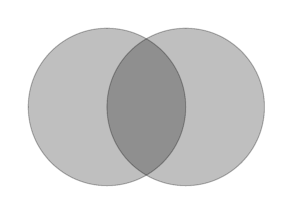
\begin{tikzpicture}
\draw[fill=black, opacity=0.25, color=black] (0,0) circle (1);
\draw[fill=black, opacity=0.25, color=black] (1,0) circle (1);
\end{tikzpicture}\\
\textit{Proof} In general, $\mathbf{P}[A \cup B] \leq \mathbf{P}[A] + \mathbf{P}[B]$. Let's test our particular case:  \\ \\
$1 = \mathbf{P}[(X \leq \mathbb{E}[X]) \cup (X \geq \mathbb{E}[X])] \leq
\mathbf{P}[X \leq \mathbb{E}[X]] + \mathbf{P}[ X \geq \mathbb{E}[X]]  $ \\ \\
Uh...\\ \\
$1 \geq a \geq 0$ and $1 \geq b \geq 0$ and $a + b \geq 1$ we'd like to conclude $a > 0$ and $b > 0$. \\ \\
Well... \\ \\
If $b \geq 1 - a = 0$ then $a = 1$. In our case,  $\mathbf{P}[X \leq \mathbb{E}[X]] = 0$ and $\mathbf{P}[X \geq \mathbb{E}[X]] = 1$. \\ \\
That looks fine... \\ \\
$\mathbf{P}[X > \mathbb{E}[X]] = 1$ and yet $\mathbf{P}[X \geq \mathbb{E}[X]] = 1$. I'm guessing $\mathbf{P}[X = \mathbf{E}[X]] = 0$. \\ \\
Why can't $\mathbf{P}[X < \mathbb{E}[X]] = 0$? \\ \\
Our value is \textit{never} less than what we expected.  Then maybe we should set our expectations higher? \\ \\
We always have $X > \mathbb{E}[X]$ then
$$ \mathbb{E}[X] \leq \sum_{X \leq \mathbb{E}[X]} x\,\mathbb{P}[x] +  \sum_{X \geq \mathbb{E}[X]} x\,\mathbb{P}[x] = 0  +  \sum_{X >  \mathbb{E}[X]} x\,\mathbb{P}[x]  $$
if we always have $X > \mathbb{E}[X]$ then
$$ \mathbb{E}[X] \leq \sum_{X \leq \mathbb{E}[X]} x\,\mathbb{P}[x] +  \sum_{X \geq \mathbb{E}[X]} x\,\mathbb{P}[x] = \sum_{X <  \mathbb{E}[X]} x\,\mathbb{P}[x] + 0
 < \mathbb{E}[X] \; \mathbb{P}[X < \mathbb{E}[X]]$$
if we have that $\mathbb{E}[X] > 0$ then we concllude that $\mathbf{P}[X < \mathbb{E}[X]] > 1$.  Unfortunately we do not have this assumption. \hfill $\varnothing$\\ \\
\textit{Proof} How about we have that $\mathbb{E}[X - \mathbb{E}[X]] = 0$, this is called ``centering".
$$ 0 = \mathbb{E}[X - \mathbb{E}[X]] = \sum_{X \leq \mathbb{E}[X]} (x - \mathbb{E}[X])\;\mathbf{P}[x]
+ \sum_{X \geq \mathbb{E}[X]} (x - \mathbb{E}[X])\;\mathbf{P}[x]$$  
By definition of our idea of ``probability" $\mathbf{P}[x] \geq 0$ and yet the total of these numbers is zero.  Therefore some term is positive and some term is negative, we have $x > \mathbb{E}[X]$ and $x < \mathbb{E}[X]$ in some case. \\ \\
Cleainup?  Maybe using conditional probablity:
\begin{eqnarray*} 0  &=& \mathbb{E}[X - \mathbb{E}[X]] \\ 
&=& \mathbb{E}\Big[X - \mathbb{E}[X] | X \leq \mathbb{E}[X]\Big] \mathbf{P}( X \leq \mathbb{E}[X]) \\
&+& \mathbb{E}\Big[X - \mathbb{E}[X] | X \geq \mathbb{E}[X]\Big] \mathbf{P}( X \geq \mathbb{E}[X]) \\
&=& a\mathbf{P}( X \leq \mathbb{E}[X]) + b \mathbf{P}( X \geq \mathbb{E}[X])
\end{eqnarray*}
where $a \leq 0$ and $b \geq 0$.  Yet:
$$\mathbf{P}( X \leq \mathbb{E}[X]) +  \mathbf{P}( X \geq \mathbb{E}[X]) \geq 1 $$
$$ 0 = a\mathbf{P}( X \leq \mathbb{E}[X]) + b \mathbf{P}( X \geq \mathbb{E}[X])
\geq a\mathbf{P}( X \leq \mathbb{E}[X]) + b (1 -  \mathbf{P}( X \leq \mathbb{E}[X]))$$
Then maybe if we arrange more carefully:
$$ 0 \geq (a - b)\mathbf{P}(X \leq \mathbb{E}[X]) + b $$
Let's try one more:
$$ \mathbf{P}(X \leq \mathbb{E}[X]) \geq \frac{b}{b-a} $$
Maybe easier:
$$ (-a)\mathbf{P}( X \leq \mathbb{E}[X]) = b \mathbf{P}( X \geq \mathbb{E}[X])$$
Let's rule out $a = 0$ and $b = 0$.  If $a = 0$, either
\begin{itemize}
\item $\mathbf{P}(X \leq \mathbf{E}[X]) = 0$ and $P (X \geq \mathbf{E}[X]) = 1$
\item $b = 0 $
\end{itemize}
$$  \mathbb{E}\Big[X  | X \leq \mathbb{E}[X]\Big] -  \mathbb{E}[X]  = \mathbb{E}\Big[X - \mathbb{E}[X] | X \leq \mathbb{E}[X]\Big] = 0 $$
Looks like we need to consider the event $\mathbb{P}[ X = \mathbb{E}[X]] > 0$ that there is probability concentrated at one point .

Another great option is \dots our world doesn't stop because we find one or two or even a hundred contradictions.  Our logic keeps going our culture keeps going and we keep existing.  How do we humans reason in such murky and contradictoary environment? \\ \\

\newpage

\begin{thebibliography}{}

\item Terence Tao, Van Vu.  \textbf{Additive Combinatorics} Cambridge University Press. \dots 

\end{thebibliography}

\end{document}